\chapter{Marco Teórico}

En este capítulo se describen conceptos relacionados con la tarea de perfilado de autor mediante algoritmos de aprendizaje automático. Se describen las principales representaciones de un texto dado, las características generales de los clasificadores empleados, así como las medidas de evaluación empleadas para medir los resultados de los diferentes modelos. Además se presenta una introducción de las  tareas de procesamiento de lenguaje natural utilizadas en el método propuesto: etiquetado de partes de la oración, paráfrasis y resolución de analogías.

\section{Clasificación de textos}

En años recientes, ha habido un crecimiento exponencial en el número de textos disponibles en Internet, a tal grado que es imposible procesarlos manualmente, de ahí la importancia de su procesamiento automático. Los problemas de clasificación automática de textos han sido ampliamente estudiados en las últimas décadas, especialmente con los avances en procesamiento de lenguaje natural, muchos investigadores están interesados en desarrollar aplicaciones que mejoren los métodos de clasificación de textos. Las tareas exploradas en este trabajo se circunscriben a las tareas de perfilado de autor, donde se desea conocer la categoría (clase o tipo de autores) a la que pertenece un documento dado (historial del usuario).

\subsubsection{Definición}

La clasificación de textos puede ser definida como la tarea de categorizar un grupo de documentos en una o más clases predefinidas de acuerdo con sus temas \citep{Kadhim2019}. Retomando la definición de \citep{Kadhim2019}, se parte con un grupo específico de documentos $D={\begin{Bmatrix} d_1 , ... , d_n \end{Bmatrix}}$, con clases predefinidas $C={\begin{Bmatrix} c_1 , ... , c_m \end{Bmatrix}}$ y un nuevo documento $q$ el cual es generalmente indicado como una consulta, con el objetivo de predecir la clase del documento consultado, la cual puede ser una o más clases pertenecientes a $C$.

De acuerdo con \citep{kowsari2019text}, la clasificación de textos puede describirse en cuatro pasos: extracción de características, reducción de dimensionalidad o selección de características, construcción del modelo de clasificación y evaluación. A continuación, se describen en forma resumida algunos de los puntos más importantes para este trabajo, tomados del análisis de \citep{kowsari2019text}.

\section{Extracción de características}
El pre-procesamiento y la extracción de características son pasos muy importantes en la clasificación de textos, en las siguientes secciones se presentan algunas de las técnicas más empleadas y se mencionan dos métodos de representación de características: la bolsa de palabras y las representaciones distribucionales.

\subsection{Pre-procesamiento}
Dependiendo de la tarea de clasificación, algunos elementos pueden desecharse para enfocar nuestra atención en los elementos más informativos. Algunos de estos elementos son: palabras de paro, errores gramaticales, signos de puntuación, etc. Además de esto, el texto extraído de redes sociales contiene enlaces de internet, menciones de usuario, etiquetas (conocidos como hashtags), emoticonos y un vocabulario muy informal (p.e. abreviaturas no convencionales).  A continuación se explica brevemente algunas técnicas empleadas para el limpiado y pre-procesamiento de textos.

\begin{enumerate}
\item \textbf{Tokenización}: Es un método de pre-procesamiento en el cual se divide una cadena de caracteres en palabras, frases, símbolos y otros elementos dentro del texto llamados \textit{tokens} \citep{kowsari2019text}. Se pueden utilizar diferentes algoritmos para poder realizarlo lo más simple es separar el texto mediante un espacio o caracter común, por ejemplo:

Texto original: \textit{``Los días de verano son calurosos''}.

Los tokens del texto anterior son los siguientes: \{``Los'',  ``días'', ``de'', ``verano'', ``son'', ``calurosos''\}'

\item \textbf{Palabras de paro}: Son palabras con mayor frecuencia en los documentos, y por lo tanto poco útiles para la discriminación entre documentos de diferentes clases. Ejemplos de ellas son: \{``\textit{a}'' ``\textit{the}'', ``\textit{they}'', ``\textit{he}'' , ``\textit{she}'', ...\} (para el idioma Inglés). En algunas tareas de clasificación de textos las palabras de paro no son de importancia y lo más común es removerlas de los documentos o textos. Nothman \citep{nothman2018stop} presenta un análisis de las palabras de paro.

\item \textbf{Capitalización}: Los textos contienen diversas formas de capitalización de palabras para formar una oración. Dado que los documentos consisten en muchas oraciones, una capitalización diversa puede ser muy problemática en la clasificación de textos largos. La técnica más común para tratar la capitalización inconsistente es reducir cada palabra a minúsculas \citep{kowsari2019text}.

\item \textbf{Reducción de ruido}: La mayoría de los textos contienen caracteres innecesarios para la clasificación de documentos, como signos de puntuación o caracteres especiales. En tareas como detección de autoría pueden ser útiles pero en general agregan ruido a los modelos de clasificación de textos.

\item \textbf{Stemming}: Es el proceso de convertir palabras a su forma base o raíz  (e.g., morfema base del significado) \citep{kamath2019deep}. Uno de los algoritmos más populares es el algoritmo de Poter \citep{porter2001snowball}.

\item \textbf{Lematización}:  Es el proceso de convertir palabras a su forma base o raíz, a diferencia del proceso de stemming es que en este proceso el significado y el contexto puede ser conservado. La desventaja es que este método requiere un diccionario y tablas de búsqueda \citep{kamath2019deep}.

\item  \textbf{Otras técnicas}: Adicionalmente a  las técnicas descritas también es posible pre-procesar los textos para intentar normalizarlos con la intención de facilitar al clasificador la identificación de patrones. Algunas de ellas son: la corrección de errores ortográficos, enmascaramiento de textos, etiquetado de partes de la oración, etc.

\end{enumerate}


\subsection{N-Gramas}
Es una técnica para extraer características para representar un texto, los n-gramas son un conjunto de palabras o caracteres que respetan el orden de aparición en el texto; el número $n$ indica la longitud de la secuencia a considerar, lo más común es utilizar valores de $n$ pequeños (uni-gramas, bi-gramas, tri-gramas) \citep{kowsari2019text}. 

\textbf{Ejemplo de bi-gramas}: 

Texto Original: \textit{``Con el tiempo todo pasa''}

Bi-gramas:\{``con el", ``el tiempo", ``tiempo todo", ``todo pasa"\}


\subsection{Bolsa de palabras BoW}
El modelo de bolsa de palabras o BoW (por sus siglas en inglés ``Bag of Words'') es una representación simplificada de un texto. Normalmente, se utiliza un criterio o pesado específico, como lo puede ser la frecuencia de cada palabra, para representar cada texto . Es decir, en el modelo BoW, el conjunto de documentos es representado mediante una matriz de pesos, siendo las columnas palabras únicas del conjunto de datos y las filas representan un documento. Este modelo es muy simple, donde no es posible capturar el orden secuencial de las palabras -como en una oración o un documento-, con lo que las relaciones semánticas entre las palabras se pierden. Sin embargo, en este modelo las palabras capturan el contenido de un documento y esta representación puede ser utilizada para determinar el tema principal de dicho documento \citep{kowsari2019text}.


%\textbf{Ejemplo de BoW}

%\textbf{Texto original}: `` \textit{Informalmente, un algoritmo es cualquier procedimiento computacional bien definido que recibe algún valor, o conjunto de valores, como entrada y produce un valor, o conjunto de valores, como salida. Un algoritmo es entonces un conjunto de pasos computaciones que transforman la entrada en la salida.}''

%\textbf{Bolsa de palabras}: \{procedimiento,
% valores,
% algoritmo,
% bien,
% de,
% o,
% que,
% algun,
% como,
% valor,
% salida,
% transforman,
% pasos,
% recibe,
% computaciones,
% computacional,
% ,,
% Un,
% la,
% definido,
% cualquier,
% en,
% Informalmente,
% es,
% produce,
% .,
% un,
% entonces,
% entrada,
% conjunto,
% y\}

% \textbf{Pesos para el documento ejemplo}: [1, 2, 2, 1, 3, 2, 2, 1, 2, 2, 2, 1, 1, 1, 1, 1, 5, 1, 2, 1, 1, 1, 1, 2, 1, 2, 3, 1, 2, 3, 1]

\subsubsection{Pesado de palabras}La forma más básica de pesado de características es mediante el pesado TF (\textit{term frequency} por sus siglas en inglés), el cual consiste en contar el número de ocurrencias de cada palabra en el conjunto de datos. Los métodos basados en TF generalmente consisten en representar la frecuencia de palabras como un peso escalado o normalizado, aunque es de fácil implementación y muy intuitivo este método está limitado por el hecho de que las palabras más comunes pueden dominar la representación.

\subsubsection{TF-IDF Term Frequency-Inverse Document Frequency} Esta técnica de  pesado fue propuesta por \citep{jones1972statistical}, con el objetivo de mitigar el efecto de las palabras más comunes en el corpus. IDF asigna menos peso a aquellas palabras que por estar presentes en la mayoría de los documentos de la colección no son útiles para identificar patrones discriminativos. La representación matemática del peso de un término en un documento por TF-IDF está dada en la ecuación \ref{eq:tf_idf}

\begin{equation}
W(d, t) =T F(d, t) * log(N/df(t))
\label{eq:tf_idf} 
\end{equation}

En donde $N$ es el número total de documentos en la colección y $df(t)$ es el número de documentos que contienen el término $t$, el primer término $TF(d,t)$ es la frecuencia del término $t$ en el documento $d$. Aunque TF-IDF trata de solucionar el problema de términos comunes en el documento, sigue sufriendo de otras limitaciones. Un problema común es que TF-IDF no se puede utilizar para medir la similitud entre palabras en el documento, dado que cada palabra es independiente representada por un índice.

\subsection{Representaciones distribucionales}
Su principal objetivo es capturar el significado semántico de las palabras, en donde cada palabra del vocabulario es representada mediante un vector n-dimensional de números reales. Recientemente \citep{mikolov2013distributed} presentó el modelo Word2Vec, para generar vectores de palabras, el cual tiene dos algoritmos: el modelo CBOW y el modelo Skip-gram respectivamente. CBOW  predice la palabra central del contexto que la rodea, mientras que Skip-gram hace lo contrario y predice la distribución (probabilidad) de las palabras de contexto de una palabra central. Word2Vec proporciona una herramienta muy poderosa para descubrir relaciones entre los textos de un corpus así como la similitud entre palabras.

%Poner un diagrama
%\subsection{Glove}
Es un modelo similar Word2Vec, fue propuesto por \citep{pennington2014glove} y su objetivo principal de capturar contextos globales combinando factorización de matrices y ocurrencias locales. Este modelo demostró ser más rápido en entrenamiento y mejora en tareas como analogía (en comparación con Word2Vec). Los autores generaron diferentes modelos pre-entrenados para su libre acceso, estos modelos fueron entrenados sobre grandes conjuntos de datos como CRAWL\footnote{www.commoncrawl.org} y Wikipedia\footnote{www.wikipedia.org}.

%\subsection{FastText}
Otro modelo distribucional es el llamado FastText. Este modelo fue desarrollado por el laboratorio de inteligencia artificial de Facebook \citep{mikolov2017advances}. A diferencia de los modelos anteriores este modelo considera la morfología de las palabras, cada vector es enriquecido con una bolsa de vectores de caracteres de n-gramas que es derivada de una matriz de co-ocurrencia. La  principal ventaja de este modelo es su habilidad de obtener vectores para palabras fuera del vocabulario. Los vectores pre-entrenados están disponibles en la página oficial de FastText\footnote{www.fasttext.cc}  y la última liberación fue un modelo entrenado en 157 idiomas \citep{grave2018learning}.

Para un mayor detalle de la teoría y el cálculo de este tipo de representaciones consultar el capítulo 5 del libro de \citep{kamath2019deep}.
\section{Selección de características}

Un problema común en la clasificación de textos es el manejo de grandes espacios vectoriales (cientos de miles dependiendo de la extracción utilizada) y como consecuencia se necesita grandes cantidades de memoria y tiempo de computación para poder procesar los algoritmos de aprendizaje. Una solución efectiva consiste en seleccionar las características que mejor discriminan a las clases.

Existen diversos métodos para seleccionar características entre los más utilizados se encuentran:

\begin{enumerate}
    \item Umbral de Frecuencia: Se mide para cada palabra $w$ del vocabulario, el número de documentos en que $w$ aparece. Aquellas palabras poco usadas, es decir, con pocos contextos de uso se eliminan. Es de esperar, que las palabras más frecuentes también aparezcan en documentos no vistos \citep{yang1997comparative}.
    
    \item Ganancia de información: Se establecen como relevantes todas aquellas palabras con una GI mayor a cero. Esta técnica tiene un sesgo muy importante respecto al conjunto de entrenamiento, sobretodo si éste es pequeño \citep{yang1997comparative}.   
    \item Chi cuadrada: Es un test estadístico que mide la independencia entre un término $t$ y una clase $c$. Para cada término, una puntuación alta indica que la hipótesis nula de independencia debe ser rechazada y la ocurrencia del término y la clase son dependientes \citep{yang1997comparative}.
\end{enumerate}

En \citep{yang1997comparative} se encuentra la definición matemática de cada uno de los métodos y \citep{forman2003extensive} presenta un análisis más extenso junto con otros métodos. 

\section{Algoritmos de clasificación}
Se han utilizado diversos algoritmos de aprendizaje automático para la clasificación de textos, dentro de los más populares y frecuentemente utilizados como línea base son las máquinas de soporte vectorial o SVM por sus siglas en inglés. Por otro lado, respecto a las arquitecturas de aprendizaje profundo que se han empezado a emplear, se distinguen dos arquitecturas básicas: las redes recurrentes y las redes convoluciones. En esta sección se explican las generalidades de estos algoritmos. En \citep{Minaee2020} se puede encontrar una revisión más detallada del estado del arte en la clasificación de textos con aprendizaje profundo.


\subsection{Máquinas de Soporte Vectorial (SVM)}
Este algoritmo de clasificación fue propuesto por \citep{vapnik1964class}, desde entonces el algoritmo ha pasado por una serie de mejoras. \citep{boser1992training} adaptó el algoritmo para resolver problemas no lineales  y la formulación moderna fue desarrollada por \citep{cortes1995support}.

Retomando las definiciones de \citep{boser1992training}, SVM encuentra una función de decisión para vectores $x$ de características de dimensión $n$ pertenecientes a alguna clase A o B. La entrada al algoritmo de entrenamiento es un conjunto de $p$ ejemplos $x_i$ con etiquetas $y_i$:

\begin{equation} \label{eq:training}
(x_1, y_1), (x_2, y_2), (x_3, y_3), ... , (x_p, y_p) 
\end{equation}

\[
    \text{donde}
    \begin{cases}
        y_k=1 & \text{si $x_k \in A$}\\
        y_k=-1 & \text{si $x_k \in B$}
    \end{cases}
\]

Para los ejemplos de entrenamiento el algoritmo encuentra una función de decisión $D(x)$ durante una fase de aprendizaje. Después del entrenamiento, la clasificación de patrones desconocidos es predicha de acuerdo a la siguiente regla:

\begin{equation} \label{eq:svm_de}
\begin{split}
    x \in A \text{ si } D(x)>0 \\
    x \in B \text{ si no } 
\end{split}
\end{equation}

Las funciones de decisión deben ser lineales en sus parámetros pero no están restringidas a dependencias lineales de $x$. Estas funciones pueden ser expresadas idénticamente a un \textit{perceptron }\citep{block1962analysis}:

\begin{equation} \label{eq:percetron}
    D(x) = \sum_{i=1}^{N} w_i\phi_i(x) + b
\end{equation}

En la ecuación \ref{eq:percetron} $ \phi_i$ son funciones predefinidas de $x$ y $w_i$ y $b$ son los parámetros ajustables a aprender.

En la formulación de \citep{boser1992training, cortes1995support} podemos encontrar como aproximar este tipo de funciones construyendo hiperplanos separados que maximicen un margen, mediante algoritmos de optimización numérica. \\

Las ventajas\footnote{Listadas en https://scikit-learn.org/stable/modules/svm.html} de SVM son: 
\begin{itemize}
    \item Son efectivas en espacios altamente dimensionales, como es el caso en la clasificación de textos.
    \item Son efectivas en casos en donde el número de dimensiones es mayor al número de ejemplos.
    \item Usa un subconjunto de puntos de entrenamiento en la función de decisión llamados vectores de soporte, así que es también eficiente en el uso de la memoria.
    \item Se pueden especificar diferentes funciones de núcleo para la función de decisión. 
\end{itemize}

Las desventajas incluyen:
\begin{itemize}
    \item Si el número de características es mucho mayor al número de ejemplos, elegir una función de núcleo y término de regularización es crucial para evitar el sobre ajuste.
    \item Las SVMs no otorgan directamente estimaciones de probabilidad, éstas son calculadas utilizando validación cruzada.
    
\end{itemize}
    
    
    
%\subsubsection{C-SVM}

\subsection{Redes neuronales profundas}

En la definición de \citep{lecun2015deep}, el aprendizaje profundo permite a los modelos computaciones que están compuestos de múltiples capas de procesamiento aprender representaciones de los datos con múltiples niveles de abstracción. Estos métodos han mejorado dramáticamente el estado del arte en el varias tareas en el entendimiento de lenguaje natural, particularmente, clasificación de textos, análisis de sentimientos, respuesta a preguntas y traducción automática. El aprendizaje profundo descubre estructuras en grandes conjuntos de datos utilizando el algoritmo de retro-propagación para determinar sus parámetros internos que son utilizados para calcular la representación en cada capa de la arquitectura.

A continuación se describen los conceptos principales en aprendizaje profundo tomados principalmente de \citep{lecun2015deep}, para una definición mas extensa consultar \citep{kamath2019deep, goodfellow2016deep}.

\subsubsection{Retropropagación y entrenamiento de arquitecturas multicapa}

Una arquitectura multicapa es una pila de modelos simples y muchos de éstos calculan un mapeo entrada-salida no lineal. El procedimiento de retro-propagación que calcula el gradiente de una función objetivo con respecto a los pesos de múltiples capas es una aplicación práctica de la regla de la cadena para derivadas.

Las arquitecturas multicapa aprenden a mapear una entrada de tamaño fijo (por ejemplo, la representación vectorial de un documento) a una salida de tamaño fijo (por ejemplo, las categorías de documentos). Para ir de una capa a la siguiente, un conjunto de unidades (nodos o neuronas) calculan una suma pesada de las entradas de la capa anterior y el resultado es pasado a través de una función no lineal. A la fecha, la función ReLU (\ref{eq:RELU})  es una de las más populares ya que se ha demostrado empíricamente que permite aprender más rápido en redes neuronales con muchas capas \citep{glorot2011deep}. Las neuronas que no forman parte de la capa de entrada ni la de salida se conocen como unidades ocultas. 

Las\textbf{ capas ocultas} pueden ser vistas como una distorsión de la entrada en una forma no lineal para que las categorías sean linealmente separables por la última capa.

\begin{equation} \label{eq:RELU}
    f(z)= max(z,0)
\end{equation}

La \textbf{capa de entrada} puede ser construida vía pesado TF-IDF, vectores de palabras o alguna otra característica o representación. En la clasificación de documentos usualmente la capa de entrada recibe un documento en representación vectorial (\ref{eq:vectorspace}).

\begin{equation} \label{eq:vectorspace}
d_{j} = (w_{1,j},w_{2,j},...,w_{i,j}...,w_{l_{j},j})
\end{equation}

En donde $l_{j}$ es el tamaño del documento $j$, y $w_{i,j}$ es la representación vectorial de la palabra $i$ en el documento $j$.

En la \textbf{capa de salida} el numero de neuronas es igual al número de clases para clasificaciones con más de dos clases y una para clasificación binaria, es la encargada de realizar la predicción final en base a las representaciones capturadas por la red neuronal.

La \textbf{inicialización} de los pesos y sesgo (bias) por lo general es con ceros o números generados con base en algún criterio, un algoritmo común de idealización es el conocido como inicialización Glorot o Xavier \citep{glorot2010understanding}, el cual es basado en números aleatorios extraídos de una distribución de probabilidad uniforme.

Cuando se entrena una red neuronal, la propagación hacia adelante es realizada en lotes o \textbf{batch} (un número de instancias de entrenamiento determinado por el hiper-parámetro llamado tamaño de batch), después se calcula el error para cada neurona mediante retro-propagación en el mismo lote. 

Una \textbf{época} es una sola iteración sobre todo el conjunto de datos, el número de épocas es un hiper-parámetro que determina cuantas veces el algoritmo de aprendizaje itera sobre todo el conjunto de entrenamiento.

%\subsubsection{Regularización}
%L1 , L2, Batch, Augment , Drotout

%\subsubsection{Optimización}
% Adam, cross-entropy, loss 

%Durante la fase de entrenamiento 

%%Agregar algunas imagenes chidas del paper de Lecun 2015


\subsubsection{Redes Neuronales Recurrentes (RNN)}
Los modelos basados en RNNs tienen el objetivo principal de capturar la dependencia entre palabras y la estructura del texto para clasificación de textos \cite{goodfellow2016deep}.

La redes recurrentes procesan una secuencia $u_t$ como entrada, un elemento a la vez, manteniendo en sus neuronas ocultas un  ``vector de estado" $x_t$ que implícitamente contiene información acerca de todos los elementos anteriores a la secuencia procesada \cite{lecun2015deep}. La formulación general de este concepto es presentado en la ecuación \ref{eq:rrn}, en donde $x_t$ es el vector de estado en tiempo $t$ y $u_t$ se refiere a la entrada en el paso $t$.


\begin{equation} \label{eq:rrn}
    x_t = F(x_{t-1}, u_t, \theta )
\end{equation}


Las redes recurrentes son sistemas dinámicos muy poderosos, pero su entrenamiento es muy problemático dado que su gradiente al ser retro-propagado crece o disminuye en cada paso, así que sobre cada paso típicamente explotan o desaparecen \citep{lecun2015deep}, para tratar de solucionar este problema se propuso un tipo especial de red recurrente conocida como LSTM.

\subsubsection{LSTM}
Propuestas originalmente por \citep{hochreiter1997long} para tratar los problemas de explotación y desvanecimiento de gradientes en redes recurrentes, las redes de memoria a corto y largo plazo son un tipo especial de red recurrente que conserva las dependencias largas de maneras más efectivas en comparación con una red recurrente básica. Las redes LSTM usan múltiples capas para regular el monto de información que será permitida en cada estado de nodo. La figura \ref{fig:LSTM} muestra la estructura interna de una celda de una LSTM. En donde $x_t$, $o$ y $h_t$ representan la entrada, salida y el estado oculto en tiempo $t$. $c_{t-1}$ es la información llevada del estado $t-1$ al estado $t$, el cual será combinado con la entrada $x_t$ y el estado oculto $h_{t-1}$ para formar el estado oculto $h_t$ y el arrastre de $c_t$ el cual será enviado al siguiente paso.

\subsubsection{Redes recurrentes bi-direccionales}
Las redes recurrentes convencionales consideran una estructura causal, significando que cada estado en tiempo $t$ captura solo información del pasado, $x,..., x^{t-1}$, y la entrada actual $x^t$. Sin embargo en muchas aplicaciones para realizar una predicción de $y^t$ que dependa de la secuencia entera, las RNNs bidireccionales fueron propuestas para resolver ese problema  \citep{schuster1997bidirectional}. Las RNNs bidireccionales combinan una red recurrente que se mueve hace adelante en el tiempo, comenzando desde el inicio del texto, con otra que se mueve hacia adelante en el tiempo, comenzando desde el fin del texto, para obtener una representación final se combina la red hacia adelante y hacia atrás mediante alguna operación con tensores (suma, concatenación, multiplicación o promedio). 



\begin{figure}[!t]
\centering
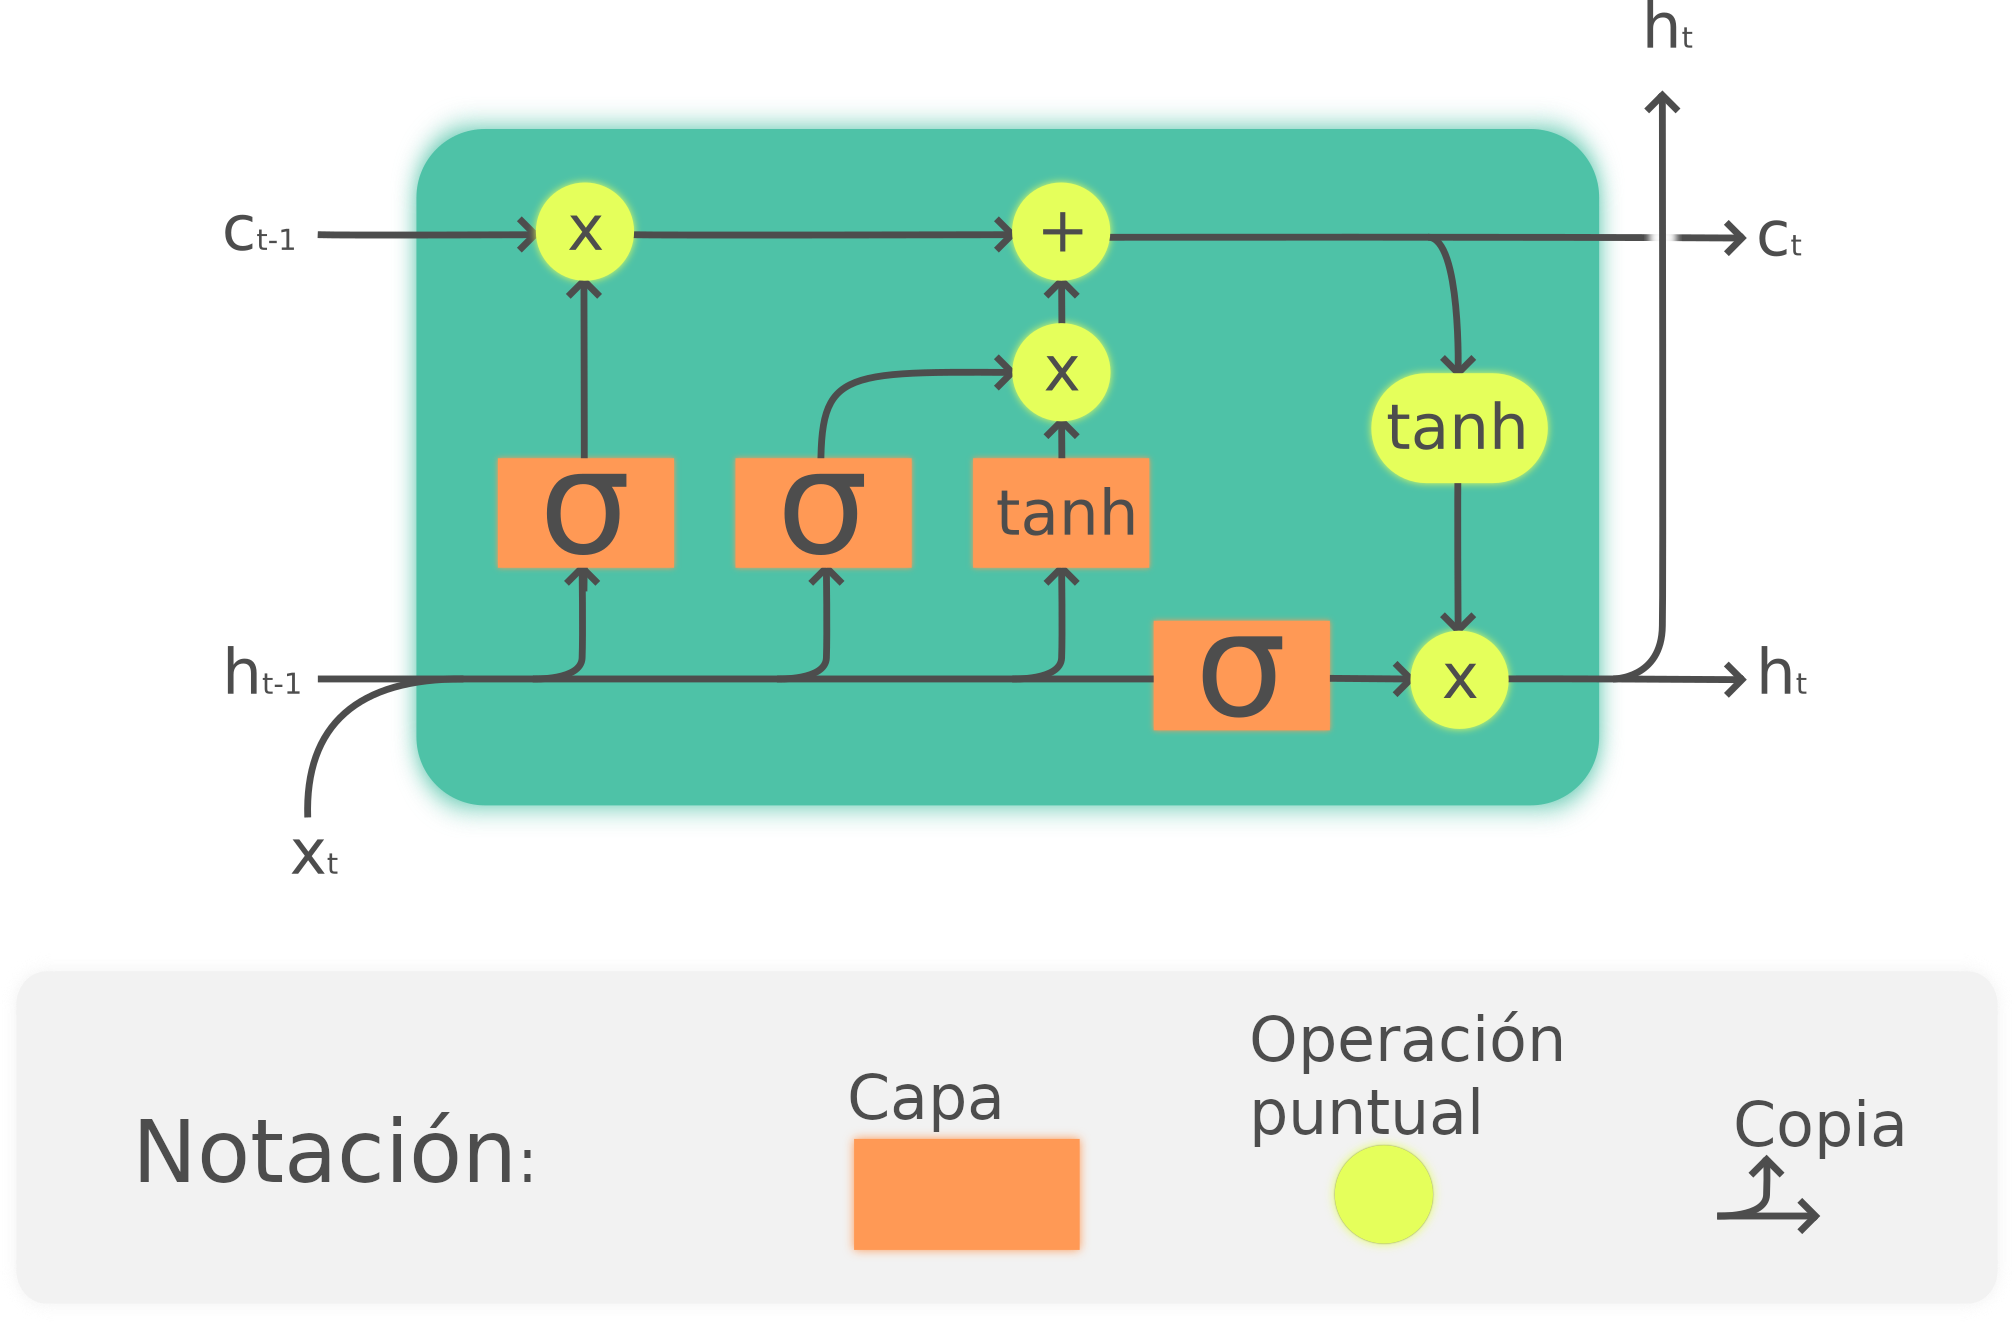
\includegraphics[width=0.7 \textwidth]{sections/figures/LSTM_cell2.png}
\caption{Una celda de LSTM desdoblada sobre el tiempo.} \label{fig:LSTM}
\end{figure}


\subsubsection{Redes Neuronales Convolucionales (CNN)}
Aunque originalmente fueron diseñadas para reconocimiento de caracteres en imágenes, las redes convolucionales han sido empleadas efectivamente para clasificación de textos \citep{kim2014convolutional, zhang2015character, zhang2015sensitivity, conneau2016very}.
En el contexto de clasificación de textos el principal objetivo de este tipo de redes es capturar un contexto local de las palabras en el documento, mediante la aplicación de un conjunto de núcleos de tamaño $d$x$d$. Estas capas de convolución son llamadas mapas de características y pueden ser apiladas para proporcionar múltiples filtros de la entrada. Para reducir la complejidad computacional, las CNNs utilizan una operación llamada pooling la cual reduce el tamaño de la salida de una capa a la siguiente en la red. Existen diferentes técnicas de pooling para reducir la salida y conservar características importantes. El pooling más empleado es el método de max pooling, el cual selecciona el elemento máximo en la ventana de pooling. Para pasar la salida de las capas de pooling, los mapas son \textit{aplanados} en una columna. La capa final en una CNN es típicamente una capa totalmente conectada.


%\subsection{Limitaciones del aprendizaje profundo}

\section{Medidas de Evaluación}

Existen diferentes métricas para evaluar los modelos de aprendizaje computacional, dependiendo de lo que se quiera medir algunas de las más utilizadas son: exactitud, precisión, recuerdo y F1. Para ilustrar cada una de estas métricas, se parte de la clasificación binaria como ejemplo. La tabla \ref{table:confusion}, conocida como matriz de confusión, resume los resultados de un clasificador. A continuación, se describen los principales conceptos\footnote{Tomados de https://medium.com/analytics-vidhya/complete-guide-to-machine-learning-evaluation-metrics-615c2864d916}.

\begin{table}[ht]
\caption{Matriz de confusión.}
\label{table:confusion} 
\centering 
\begin{small}
\begin{tabular}{l|c|c|}
\cline{2-3}
                                         & \multicolumn{1}{l|}{\textbf{Predicción: 1}} & \multicolumn{1}{l|}{\textbf{Predicción: 0}} \\ \hline
\multicolumn{1}{|l|}{\textbf{Real: 1}} & \textit{VP}                                 & \textit{FN}                                 \\ \hline
\multicolumn{1}{|l|}{\textbf{Real: 0}} & \textit{FP}                                 & \textit{VN}                                 \\ \hline
\end{tabular}
\end{small}
\end{table}


La matriz de confusión no es una medida como tal, pero las métricas de evaluación están basados en los números dentro de esta.


%\textbf{Términos asociados a la matriz de confusión:}

\begin{enumerate}
    \item \textbf{Verdaderos Positivos (VP)}: Es el número total de predicciones en que la clase real es 1 (positiva) y la predicción también es 1 (positiva).
    \item \textbf{Verdaderos Negativos (VN)}: Es el número total de predicciones en que la clase real es 0 (negativa) y la predicción también es 0 (negativa).
    \item \textbf{Falsos Positivos (FP)}: El número de predicciones en que la clase verdadera es 0 y la predicción es 1:
    \item \textbf{Falsos Negativos (FN)}: Es el número de predicciones en que la clase verdadera es 1 y la predicción es 0.
\end{enumerate}

El escenario ideal sería que el modelo obtenga $0$ falsos positivos y falsos negativos, pero ese no es el caso en la vida real y el objetivo en ocasiones es tratar de minimizar los falsos positivos o los falsos negativos.

\textbf{Exactitud}: La proporción del número de ejemplos en el conjunto de evaluación que son correctamente clasificados por el modelo. La exactitud es utilizada cuando las clases tienen la misma importancia para la clasificación.

\begin{equation} \label{eq:acc}
Exactitud = \frac{VP + VN}{VP + VN+ FN+FP}    
\end{equation}

\textbf{Precisión}: Es la proporción del número de instancias positivas predichas correctamente.

\begin{equation} \label{eq:precc}
\text{Precisión} = \frac{VP}{VP+FP}    
\end{equation}

\textbf{Recuerdo}: Representa la proporción de las instancias positivas que lograron ser recuperadas.

\begin{equation} \label{eq:recc}
\text{Precisión} = \frac {VP}{VP+FN}    
\end{equation}

\textbf{Medida F1}: Es el promedio armónico de precisión y recuerdo. Proporciona una puntuación más realista al considerar a la precisión y el recuerdo.

\begin{equation} \label{eq:f1}
F_1= \frac{2 * precision * recuerdo}{precision+recuerdo}   
\end{equation}

